\documentclass{article}
\usepackage[utf8]{inputenc}
\usepackage{polski}
\usepackage{babel}
\usepackage{graphicx}
\usepackage[margin=1in]{geometry}
\documentclass{article}
\usepackage[utf8]{inputenc}
\usepackage[utf8]{inputenc}
\usepackage{polski}
\usepackage{babel}
\usepackage{hyperref}
\usepackage{graphicx}
\renewcommand{\figurename}{Wykres}
\title{\vspace{4cm} \textbf{Projekt ze \\ Struktur Danych i Złożoności Obliczeniowiej}}
\author{Jakub Grelowski - 262754 \\
        grupa K02-10d \\
        poniedziałek P - 11:15}
\date{4 kwietnia}



\begin{document}

\maketitle

\begin{center}

\large prowadzący: dr inż. Zbigniew Buchalski 

\vspace{1cm}

\Large \textbf{\textit{Zadanie projektowe nr 1}}     
\end{center}

\vspace{1cm}

\newpage

\tableofcontents

\newpage

\section{Wstęp}

\subsection{Cel projektu}
Celem projektu było napisanie programu umożliwiającego operacje na podstawowych strukturach danych oraz analizę czasową takich operacji. 

\subsection{Analizowane struktury danych}

\begin{itemize}
    \item Tablica dynamiczna
    \item Lista dwukierunkowa 
    \item Kopiec binarny
\end{itemize}


\subsection{Testowane operacje}
W przypadku listy oraz tablicy:
\begin{itemize}
    \item Dodawanie na początek
    \item Dodawanie na koniec
    \item Dodawanie na określony indeks
    \item Usuwanie z początku
    \item Usuwanie z końca
    \item Usuwanie z określonego indeksu
    \item Wyszukiwanie
    \item Wyświetlanie
\end{itemize}
W przypadku kopca:
\begin{itemize}
    \item Dodawanie do kopca
    \item Usuwanie z korzenia
    \item Wyszukiwanie
    \item Wyświetlanie
\end{itemize}
\newpage

\section{Złożoność obliczeniowa}
Złożoność to funkcja określająca ilość zasobów (czasowych oraz pamięciowych) wymaganych do realizacji konkretnego algorytmu. Funkcja ta zależna jest od rozmiaru wejścia algorytmu. \\

Oczekiwane złożności obliczeniowe testowanych operacji:

\begin{itemize}
    \item Tablica - Dodawanie i usuwanie w każdym miejscu tablicy - $O(n)$, szukanie - $O(n)$
    \item Lista - Dodawanie i usuwanie na początku i końcu - $O(1)$, w innym miejscu i szukanie - $O(n)$
    \item Kopiec - dodawanie i usuwanie z kopca - $O(1)$, wyszkuwianie - $O(n)$
\end{itemize}

\section{Implementacja}
Struktury zostały zaimplementowane bez pomocy zewnętrznych bibliotek w języku C++. Przechowywanym elementem jest 4-bajtowa liczba całkowita typu \textit{int}.
Program umożliwia dwa rodzaje testów:

\subsection{Testy ręczne}
Testy ręczne umożliwiają samodzielne sprawdzenie poprawności działania zaimplementowanych struktur. Za pomocą konsolowego interfejsu można przetestować każdą operację oraz wyświetlić obecny stan sprawdzanej struktury. Program umożliwia ponadto wypełnienie kontenera losowymi wartości o zadanej ilości oraz zakresie.
\subsection{Testy automatyczne}
Testy automatyczne umożliwiają sprawdzenie, ile czasu zajmuje wykonanie każdej operacji. Po wpisaniu wielkości zbioru danych wejściowych przetestowana zostanie każda struktura, po czym na ekranie konsoli pokazany zostanie czas potrzebny na wykonanie poszczególnych działań. Pomiary czasu dokonywane są w następujący sposób:
\begin{enumerate}
    \item Utwórz pustą strukturę
    \item Dodaj $x$ liczb z zakresu od 1 do $x$ do struktury
    \item Włącz zegar
    \item Wykonaj operację (np. dodaj liczbę na początek struktury)
    \item Zatrzymaj zegar
    \item Zapisz wynik
\end{enumerate}
Po wykonaniu stu takich pomiarów wyliczana jest z nich średnia arytmetyczna, która wyświetlana jest na ekranie konsoli.
Do pomiaru czasu wykorzystano funkcję \textit{QueryPerformanceCounter()}.

\newpage
\section{Wyniki pomiarów}



\subsection{Tablica dynamiczna}
\subsubsection{Tabela z wynikami}
\begin{table}[h]
\resizebox{\columnwidth}{!}{\begin{tabular}{cccccccc}
                                  & dodaj na początek          & dodaj na koniec            & dodaj do środka            & usuń z początku            & usuń z końca               & usuń ze środka             & szukaj                     \\ \cline{2-8} 
\multicolumn{1}{c|}{ilość danych} & \multicolumn{1}{c|}{$ns$}  & \multicolumn{1}{c|}{$ns$}  & \multicolumn{1}{c|}{$ns$}  & \multicolumn{1}{c|}{$ns$}  & \multicolumn{1}{c|}{$ns$}  & \multicolumn{1}{c|}{$ns$}  & \multicolumn{1}{c|}{$ns$}  \\ \cline{2-8} 
\multicolumn{1}{c|}{5000}         & \multicolumn{1}{c|}{14270} & \multicolumn{1}{c|}{15598} & \multicolumn{1}{c|}{15172} & \multicolumn{1}{c|}{17379} & \multicolumn{1}{c|}{15102} & \multicolumn{1}{c|}{14407} & \multicolumn{1}{c|}{7162}  \\
\multicolumn{1}{c|}{10000}        & \multicolumn{1}{c|}{26711} & \multicolumn{1}{c|}{27987} & \multicolumn{1}{c|}{28173} & \multicolumn{1}{c|}{25506} & \multicolumn{1}{c|}{26110} & \multicolumn{1}{c|}{27385} & \multicolumn{1}{c|}{13715} \\
\multicolumn{1}{c|}{15000}        & \multicolumn{1}{c|}{36452} & \multicolumn{1}{c|}{33565} & \multicolumn{1}{c|}{34706} & \multicolumn{1}{c|}{37486} & \multicolumn{1}{c|}{37168} & \multicolumn{1}{c|}{40974} & \multicolumn{1}{c|}{20898} \\
\multicolumn{1}{c|}{20000}        & \multicolumn{1}{c|}{51391} & \multicolumn{1}{c|}{52001} & \multicolumn{1}{c|}{51981} & \multicolumn{1}{c|}{50720} & \multicolumn{1}{c|}{48577} & \multicolumn{1}{c|}{51440} & \multicolumn{1}{c|}{24805} \\
\multicolumn{1}{c|}{25000}        & \multicolumn{1}{c|}{64950} & \multicolumn{1}{c|}{54893} & \multicolumn{1}{c|}{59477} & \multicolumn{1}{c|}{55874} & \multicolumn{1}{c|}{57573} & \multicolumn{1}{c|}{62931} & \multicolumn{1}{c|}{43472} \\ \cline{2-8} 
\end{tabular}}
\end{table}
\subsubsection{Wykresy}

\begin{figure}[h]
    \centering
    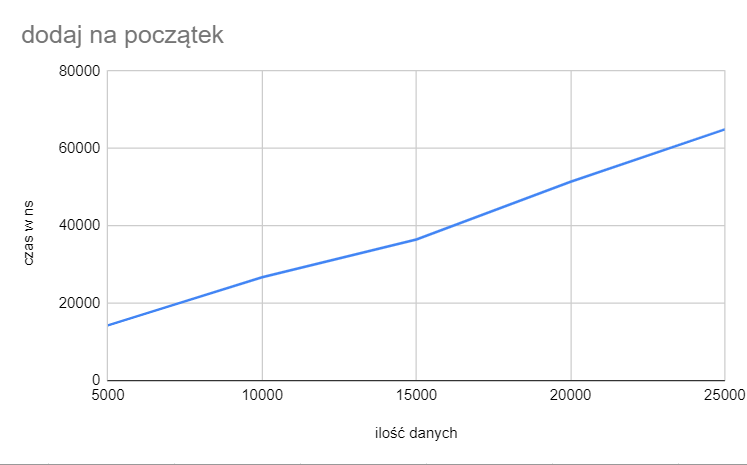
\includegraphics[scale=0.5]{images/tablica_add_to_first.png}
    \caption{Dodaj na początek - tablica}
\end{figure}
\begin{figure}[H]
    \centering
    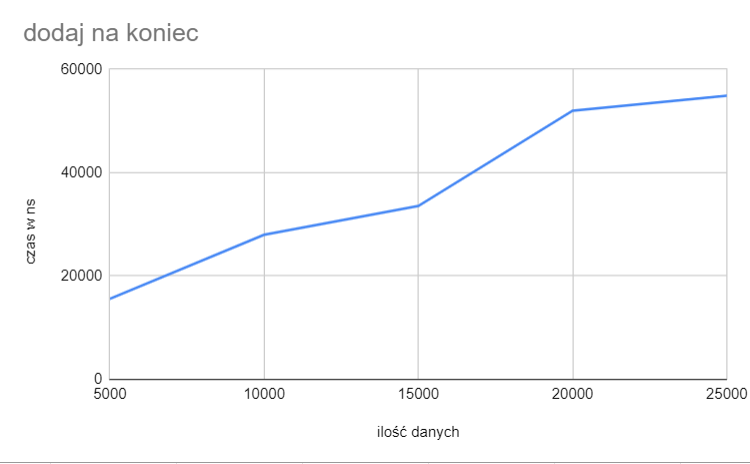
\includegraphics[scale=0.5]{images/tablica_add_to_end.png}
    \caption{Dodaj na koniec - tablica}
\end{figure}
\begin{figure}[H]
    \centering
    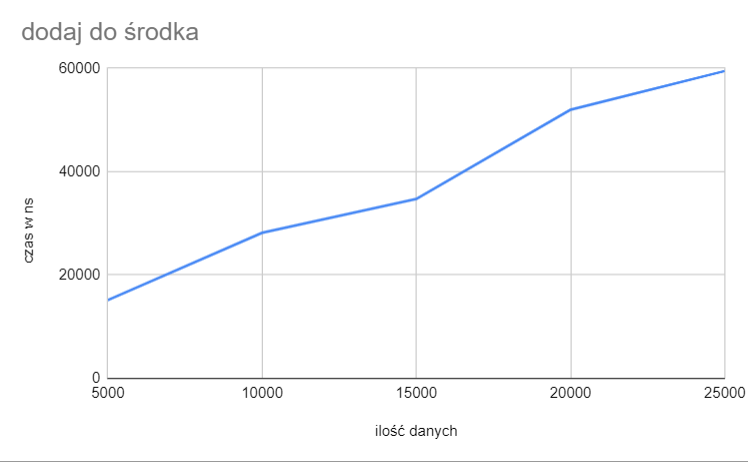
\includegraphics[scale=0.5]{images/tablica_add_to_mid.png}
    \caption{Dodaj na środek - tablica}
\end{figure}
\begin{figure}[H]
    \centering
    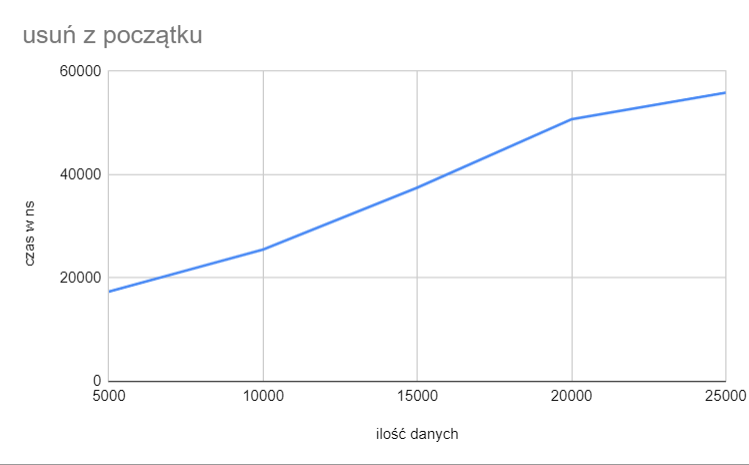
\includegraphics[scale=0.5]{images/tablica_delete_beggining.png}
    \caption{Usuń z początku - tablica}
\end{figure}
\begin{figure}[H]
    \centering
    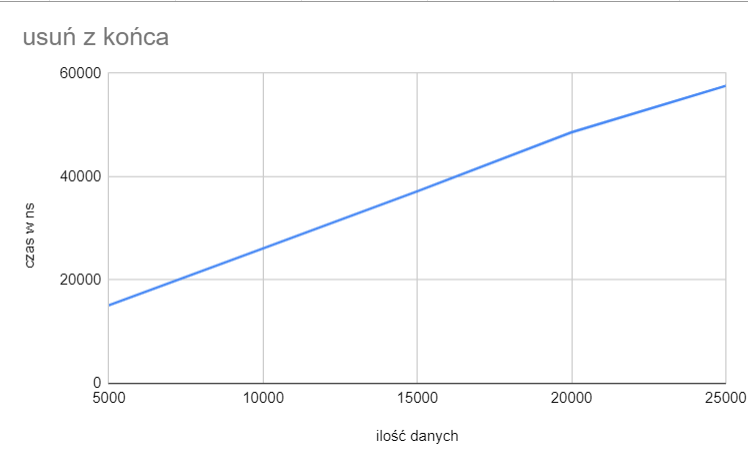
\includegraphics[scale=0.5]{images/tablica_delete_end.png}
    \caption{Usuń z końca - tablica}
\end{figure}
\begin{figure}[H]
    \centering
    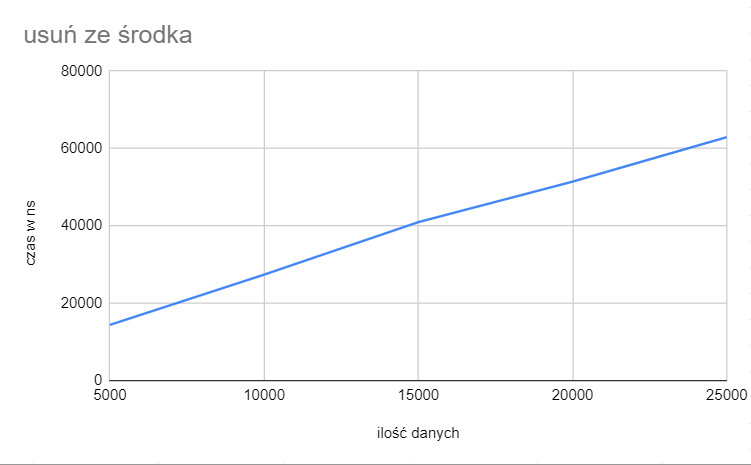
\includegraphics[scale=0.5]{images/tablica_delete_mid.png}
    \caption{Usuń ze środka - tablica}
\end{figure}
\begin{figure}[H]
    \centering
    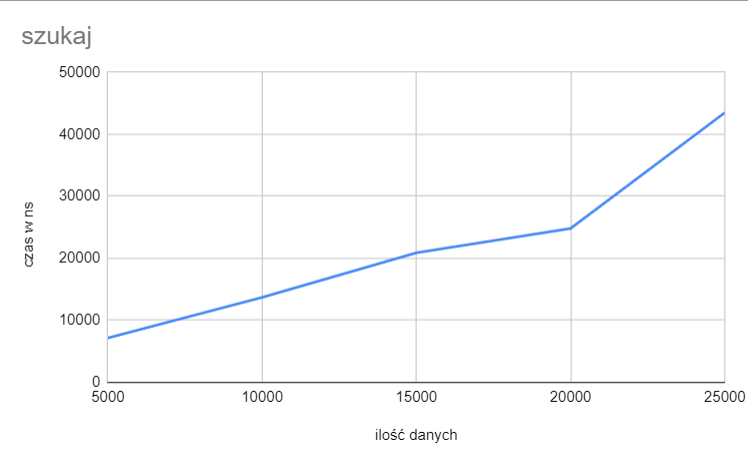
\includegraphics[scale=0.5]{images/tablica_search.png}
    \caption{Szukaj - tablica}
\end{figure}
\clearpage
\newpage
\subsection{Lista dwukierunkowa}
\subsubsection{Tabela z wynikami}
\begin{table}[h]
\resizebox{\columnwidth}{!}{\begin{tabular}{cccccccc}
                                  & dodaj na początek         & dodaj na koniec           & dodaj do środka             & usuń z początku           & usuń z końca              & usuń ze środka              & szukaj                      \\ \cline{2-8} 
\multicolumn{1}{c|}{ilość danych} & \multicolumn{1}{c|}{$ns$} & \multicolumn{1}{c|}{$ns$} & \multicolumn{1}{c|}{$ns$}   & \multicolumn{1}{c|}{$ns$} & \multicolumn{1}{c|}{$ns$} & \multicolumn{1}{c|}{$ns$}   & \multicolumn{1}{c|}{$ns$}   \\ \cline{2-8} 
\multicolumn{1}{c|}{5000}         & \multicolumn{1}{c|}{135}  & \multicolumn{1}{c|}{105}  & \multicolumn{1}{c|}{28878}  & \multicolumn{1}{c|}{61}   & \multicolumn{1}{c|}{20}   & \multicolumn{1}{c|}{36751}  & \multicolumn{1}{c|}{44715}  \\
\multicolumn{1}{c|}{10000}        & \multicolumn{1}{c|}{134}  & \multicolumn{1}{c|}{103}  & \multicolumn{1}{c|}{99500}  & \multicolumn{1}{c|}{90}   & \multicolumn{1}{c|}{30}   & \multicolumn{1}{c|}{122699} & \multicolumn{1}{c|}{125398} \\
\multicolumn{1}{c|}{15000}        & \multicolumn{1}{c|}{99}   & \multicolumn{1}{c|}{89}   & \multicolumn{1}{c|}{143585} & \multicolumn{1}{c|}{76}   & \multicolumn{1}{c|}{16}   & \multicolumn{1}{c|}{197513} & \multicolumn{1}{c|}{266981} \\
\multicolumn{1}{c|}{20000}        & \multicolumn{1}{c|}{149}  & \multicolumn{1}{c|}{140}  & \multicolumn{1}{c|}{215972} & \multicolumn{1}{c|}{116}  & \multicolumn{1}{c|}{37}   & \multicolumn{1}{c|}{293516} & \multicolumn{1}{c|}{369417} \\
\multicolumn{1}{c|}{25000}        & \multicolumn{1}{c|}{157}  & \multicolumn{1}{c|}{95}   & \multicolumn{1}{c|}{282980} & \multicolumn{1}{c|}{99}   & \multicolumn{1}{c|}{19}   & \multicolumn{1}{c|}{349771} & \multicolumn{1}{c|}{451640} \\ \cline{2-8} 
\end{tabular}}
\end{table}
\subsubsection{Wykresy}

\begin{figure}[h]
    \centering
    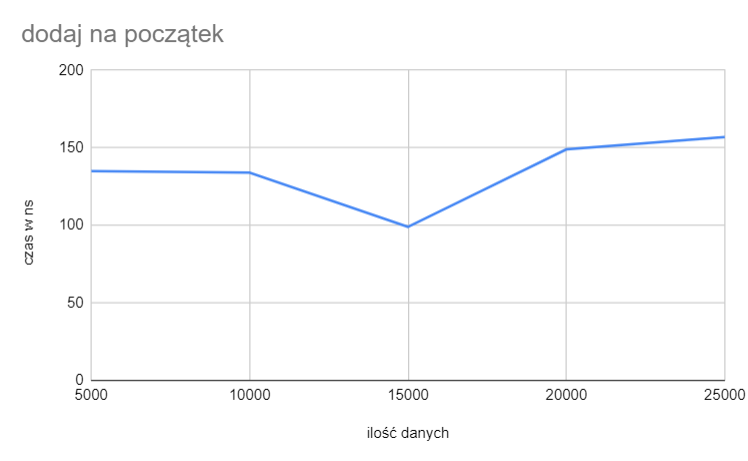
\includegraphics[scale=0.5]{images/lista_add_to_beggining.png}
    \caption{Dodaj na początek - lista}
\end{figure}
\begin{figure}[H]
    \centering
    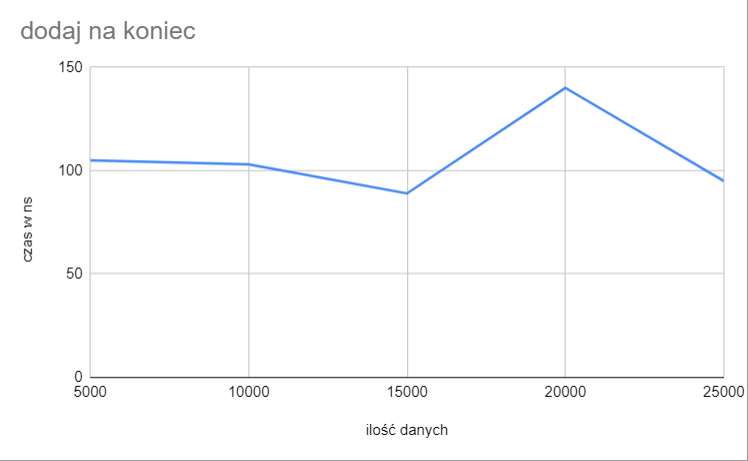
\includegraphics[scale=0.5]{images/lista_add_to_end.png}
    \caption{Dodaj na koniec - lista}
\end{figure}
\begin{figure}[H]
    \centering
    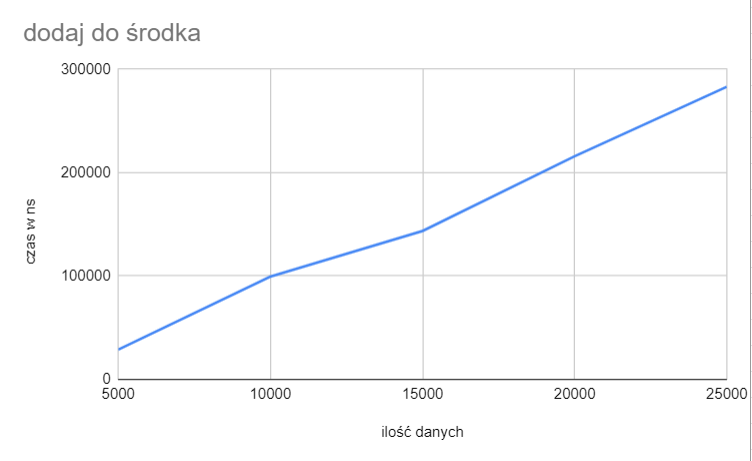
\includegraphics[scale=0.5]{images/lista_add_to_mid.png}
    \caption{Dodaj na środek - lista}
\end{figure}
\begin{figure}[H]
    \centering
    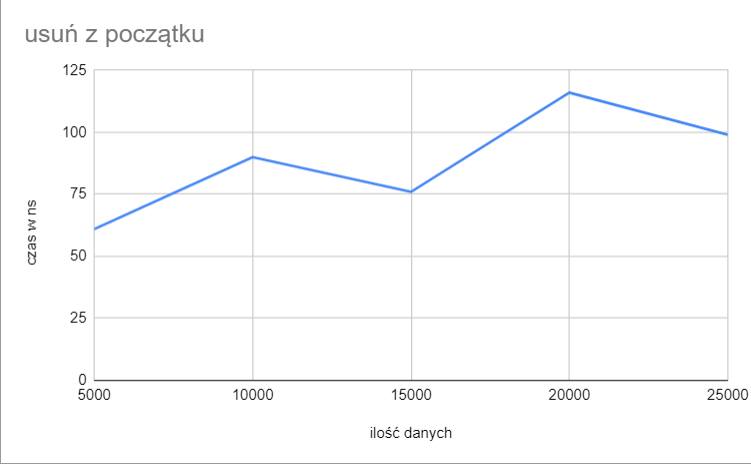
\includegraphics[scale=0.5]{images/lista_delete_beggining.png}
    \caption{Usuń z początku - lista}
\end{figure}
\begin{figure}[H]
    \centering
    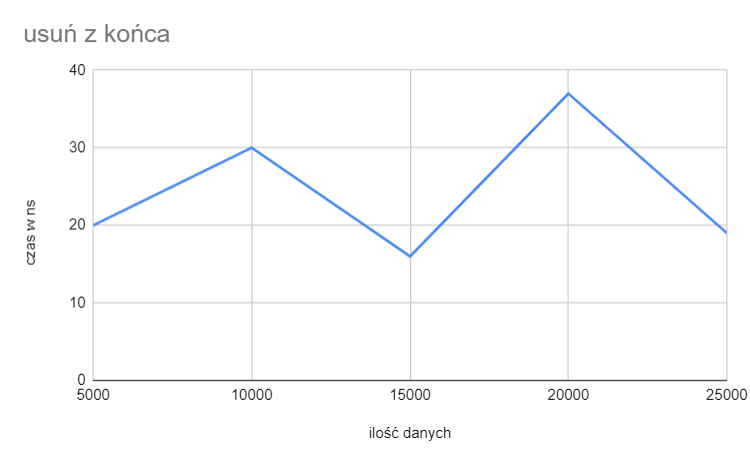
\includegraphics[scale=0.5]{images/lista_delete_end.png}
    \caption{Usuń z końca - lista}
\end{figure}
\begin{figure}[H]
    \centering
    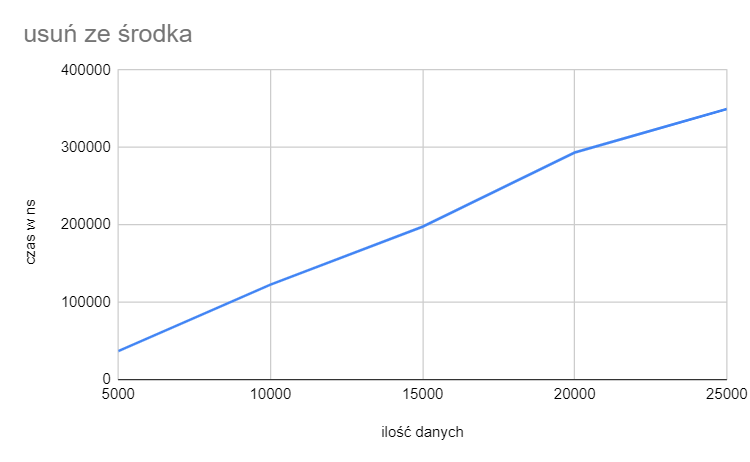
\includegraphics[scale=0.5]{images/lista_delete_mid.png}
    \caption{Usuń ze środka - lista}
\end{figure}
\begin{figure}[H]
    \centering
    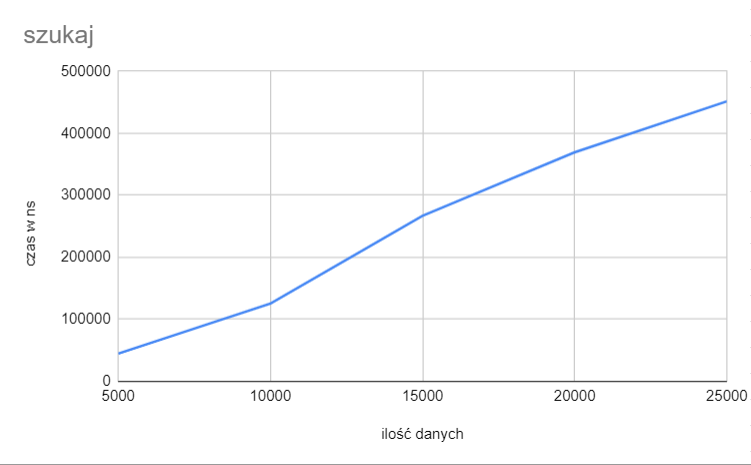
\includegraphics[scale=0.5]{images/lista_search.png}
    \caption{Szukaj - lista}
\end{figure}
\clearpage
\subsection{Kopiec binarny}
\subsubsection{Tabela z wynikami}
\begin{table}[h]
\resizebox{\columnwidth}{!}{\begin{tabular}{cccc}
                                  & dodaj do kopca             & usuń z korzenia            & szukaj                     \\ \cline{2-4} 
\multicolumn{1}{c|}{ilość danych} & \multicolumn{1}{c|}{$ns$}  & \multicolumn{1}{c|}{$ns$}  & \multicolumn{1}{c|}{$ns$}  \\ \cline{2-4} 
\multicolumn{1}{c|}{5000}         & \multicolumn{1}{c|}{13712} & \multicolumn{1}{c|}{14193} & \multicolumn{1}{c|}{3346}  \\
\multicolumn{1}{c|}{10000}        & \multicolumn{1}{c|}{27097} & \multicolumn{1}{c|}{30142} & \multicolumn{1}{c|}{12532} \\
\multicolumn{1}{c|}{15000}        & \multicolumn{1}{c|}{32667} & \multicolumn{1}{c|}{32679} & \multicolumn{1}{c|}{19139} \\
\multicolumn{1}{c|}{20000}        & \multicolumn{1}{c|}{46132} & \multicolumn{1}{c|}{51431} & \multicolumn{1}{c|}{25482} \\
\multicolumn{1}{c|}{25000}        & \multicolumn{1}{c|}{58293} & \multicolumn{1}{c|}{61501} & \multicolumn{1}{c|}{32266} \\ \cline{2-4} 
\end{tabular}}
\end{table}
\subsubsection{Wykresy}
\begin{figure}[h]
    \centering
    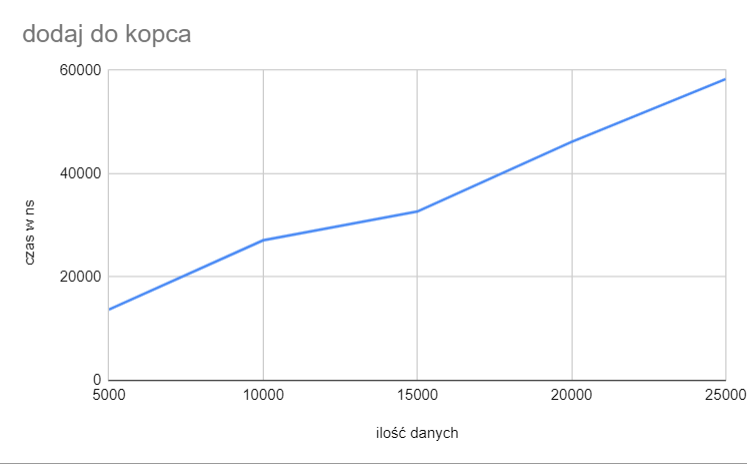
\includegraphics[scale=0.5]{images/heap_add.png}
    \caption{Dodaj do kopca}
\end{figure}
\begin{figure}[H]
    \centering
    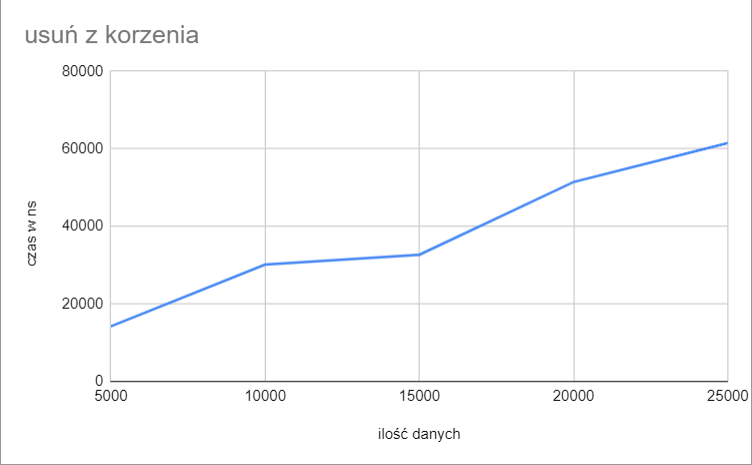
\includegraphics[scale=0.5]{images/heap_extract_max.png}
    \caption{Usuń z korzenia}
\end{figure}
\begin{figure}[H]
    \centering
    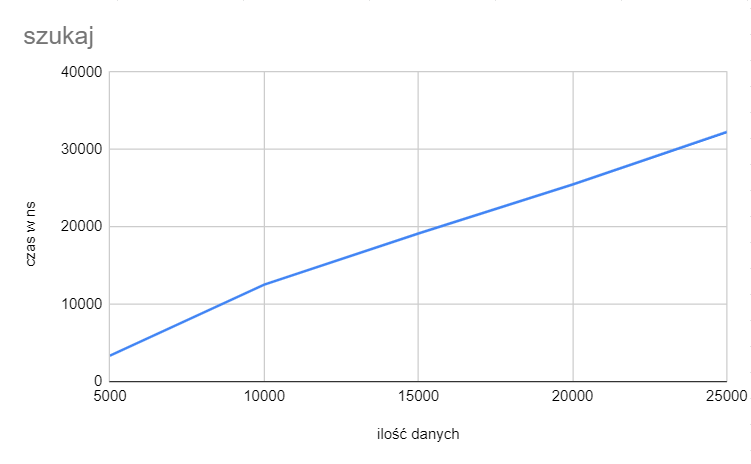
\includegraphics[scale=0.5]{images/heap_search.png}
    \caption{Szukaj w kopcu}
\end{figure}
\clearpage
\section{Wnioski}
Testowane struktury zachowywały się zgodnie z oczekiwaniami. Ich złożoności czasowe w większości zgadzają się z oczekiwanymi wartościami. \\
Porównując tablicę oraz listę można łatwo zauważyć zarówno różnice pomiędzy nimi. Tablica będzie się lepiej nadawać do wyszukiwania wartości oraz operacjach na środku struktury, natomiast lista znacznie lepiej radzi sobie z operacjami na swoim początku i końcu (metody push i pop, a także enqueue i dequeue).\\
W przypadku kopca widać różnicę pomiędzy oczekiwanymi a faktycznymi wynikami. Wynikać to może z faktu iż sam kopiec jest przechowywany w dynamicznie alokowanej tablicy. 

\end{document}